\section{Statistical Analysis and Results}


\begin{frame}{Tag and Probe}
\begin {itemize}
  \item
    Method to use Z boson to calculate efficincy of Data and Monte Carlo.
  \item
    One lepton is ``good'' (tag) and the other is used for the calculations(probe).
  \item
    Compairing Monte Carlo to data gives us Scale Factors.
\end{itemize}
\begin{center}
SuperCluster to GSF Electron\\
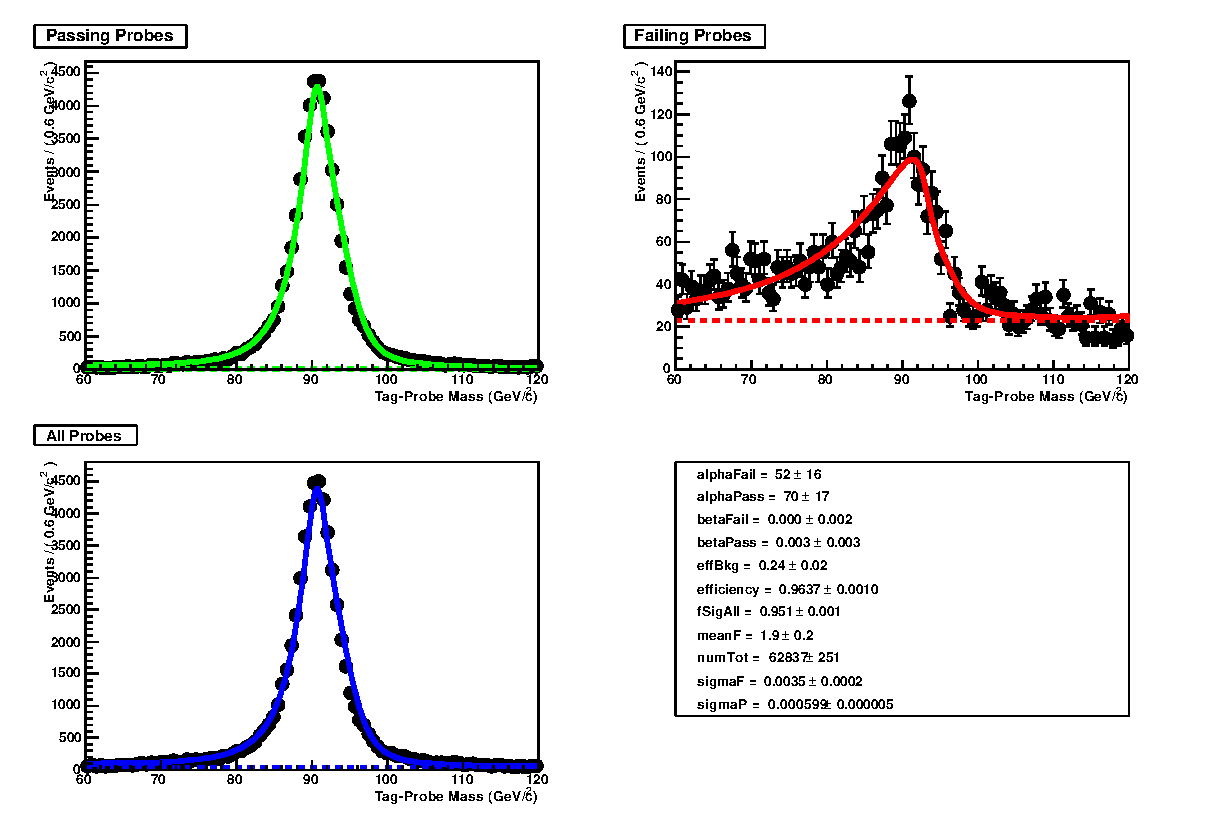
\includegraphics[width=0.49\textwidth]{images/SC_fit.eps}
\end{center}
\end{frame}


\begin{frame}{Triggers}

 % {\bf Triggers}
  \begin{columns}
    \begin{column}{0.4\textwidth}
      \begin{itemize}
      \item
        \footnotesize Muons
        \begin{itemize}
          \scriptsize
        \item
          HLT\_Mu17\_Mu8
        \item
          HLT\_Mu17\_TkMu8
        \end{itemize}
      \end{itemize}
    \end{column}
    \begin{column}{0.3\textwidth}
      \begin{center}
        {\tiny Electron Leg 8 GeV WPLoose to HLT}
        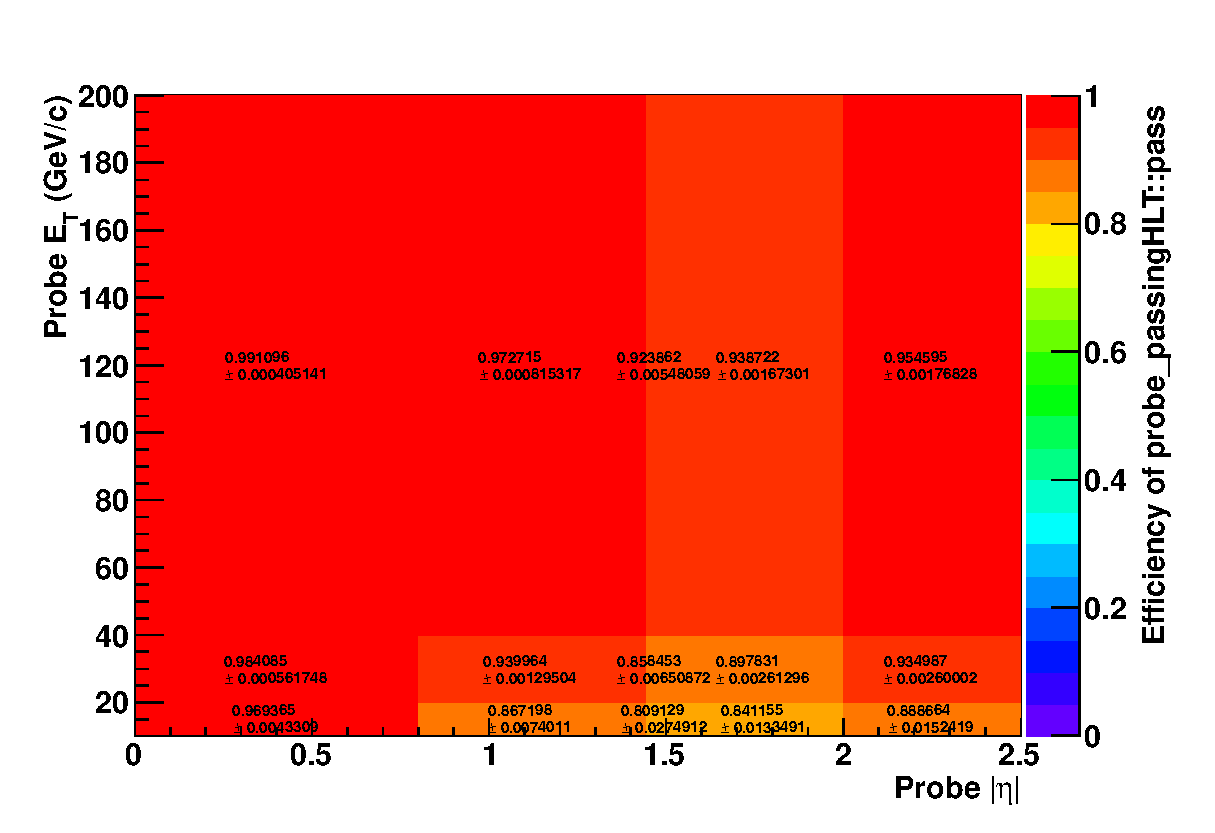
\includegraphics[width=0.99\textwidth]{images/ZJets_8.eps}
      \end{center}
    \end{column}
    \begin{column}{0.3\textwidth}
      \begin{center}
      {\tiny Electron Leg 17 GeV WPLoose to HLT}
      \includegraphics[width=0.99\textwidth]{images/ZJets_17.eps}
      \end{center}
    \end{column}
  \end{columns}
  
  \begin{columns}
    \begin{column}{1.0\textwidth}
  \begin{itemize}
  \item
    \footnotesize  Electrons
    \begin{itemize}
      \tiny
    \item
      HLT\_Ele17\_CaloIdT\_CaloIsoVL\_TrkIdVL\_TrkIsoVL \_Ele8\_CaloIdT\_CaloIsoVL\_TrkIdVL\_TrkIsoVL
    \end{itemize}
  \item
    \footnotesize EMu (for backround estimation and analysis checks)
    \begin{itemize}
      \scriptsize
    \item
      Mu8\_Ele17\_CaloIdT\_CaloIsoVL
    \item
      Mu17\_Ele8\_CaloIdT\_CaloIsoVL\_TrkIdVL\_TrkIsoVL
    \end{itemize}
  \end{itemize}
  \end{column}
    \begin{column}{0.0\textwidth}
    \end{column}
  \end{columns}

\vspace{2em}

We are using the POG provided scale factors for electrons and computing the WP to HLT ourselves. 



\end{frame}














\begin{frame}{Efficiency Fit}
The signal efficiency as a function of the Higgs mass is fitted to a polinomial in order to be estimatated for those Higgs mass hypothesis where no Monte-Carlo sample is available
\begin{center}
\includegraphics[width=0.3\textwidth]{images/plots/effFit_MU_0btag.png}
\includegraphics[width=0.3\textwidth]{images/plots/effFit_MU_1btag.png}
\includegraphics[width=0.3\textwidth]{images/plots/effFit_MU_2btag.png}
\\

\includegraphics[width=0.3\textwidth]{images/plots/effFit_ELE_0btag.png}
\includegraphics[width=0.3\textwidth]{images/plots/effFit_ELE_1btag.png}
\includegraphics[width=0.3\textwidth]{images/plots/effFit_ELE_2btag.png}





%    Electrons\\
%    \includegraphics[width=0.3\textwidth]{images/fromDani/SignalEfficiencyFits27Sept_Run2012_AB/effFit_ELE_0btag.png}
%    \includegraphics[width=0.3\textwidth]{images/fromDani/SignalEfficiencyFits27Sept_Run2012_AB/effFit_ELE_1btag.png}
%    \includegraphics[width=0.3\textwidth]{images/fromDani/SignalEfficiencyFits27Sept_Run2012_AB/effFit_ELE_2btag.png}\\
%    Muons\\
%    \includegraphics[width=0.3\textwidth]{images/fromDani/SignalEfficiencyFits27Sept_Run2012_AB/effFit_MU_0btag.png}
%    \includegraphics[width=0.3\textwidth]{images/fromDani/SignalEfficiencyFits27Sept_Run2012_AB/effFit_MU_1btag.png}
%    \includegraphics[width=0.3\textwidth]{images/fromDani/SignalEfficiencyFits27Sept_Run2012_AB/effFit_MU_2btag.png}
\end{center}
\end{frame}




\begin{frame}{Systematics}



\begin{center}
\tiny
\begin{tabular}{|l|c|c|c|p{5cm}|}
\hline
 source      &   0 $b$-tag   &   1 $b$-tag  &   2 $b$-tag  &   comment \\
\hline
%\vspace{-0.2cm}
\hline
muons  reco    &  \multicolumn{3}{|c|}{2.7\%}   &  tag-and-probe study \\
\hline
electrons reco &  \multicolumn{3}{|c|}{4.5\%}   &  tag-and-probe study  \\
\hline
jet reco             &  \multicolumn{3}{|c|}{1\%--8\%} &   JES-uncert., JER uncert. negligible; correlated between categ\\
\hline
pileup              &  \multicolumn{3}{|c|}{1-2\%}  & correlated between categ\\ %different categ quoted in Tab~\ref{tab:PU}  \\
\hline
$b$-tagging    &  2-7\%  & 3-5\% & 10-11\% & anti-correlated between categ.  \\
%\hline
%glue-tagging    & 4.6\%   & -- & -- &  loose requirement $\Rightarrow$ expected small, studies on-going \\
\hline
MET                 &  -- & -- & 3-4\% & loose requirement \\
\hline
production mechanism (PDF)&  \multicolumn{3}{|c|}{2-4\%}  & PDF4LHC, acceptance only\\
%\hline
%production mechanism (HQT)&  2\% & 5\% & 3\%  & only for $M_H=200$~GeV, $<1$\% for   $M_H=200$, $400$\\
\hline
production mechanism (WBF)&   \multicolumn{3}{|c|}{1\%} & \\
\hline
production mechanism (lineshape)&   \multicolumn{3}{|c|}{0-3\%} & only for $M_H>400$  \\
\hline
luminosity            &  \multicolumn{3}{|c|}{4.4$\%$}   & same for all analyses \\
\hline
Higgs cross-section (for $R$) &  \multicolumn{3}{|c|}{13--18$\%$ } & detailed table from YR available   \\
\hline
\end{tabular}
\end{center}
%%%%%%%%%%%%%%%%%%%%%%%%%%%%%%%%%%%%%%%%%%%%%%%%%
\end{frame}



\begin{frame}{2011 Results}
\begin{center}
\scriptsize
Limit on the expected 95$\%$ CL upper limit on the product of the Higgs boson production cross section and the branching fraction of H$\rightarrow$ZZ (black dots.), for the recorded luminosity in 2011 of 4.9 fb$^{-1}$ at 7TeV. Yellow and Green bands represent the 68$\%$ and 95$\%$ ranges of expectation.
\includegraphics[width=0.5\textwidth]{images/plots/ASCL_7TEV_unblided_new230_new_xsec.png}
\end{center}
\end{frame}



\begin{frame}{2012 Preliminary Results}
\begin{center}
\scriptsize
Limit on the expected 95$\%$ CL upper limit on the product of the Higgs boson production cross section and the branching fraction of H$\rightarrow$ZZ (dash line( and observed upper limit (black dots.) Yellow and Green bands represent the 68$\%$ and 95$\%$ ranges of expectation.
\includegraphics[width=0.5\textwidth]{images/plots/ASCL_8TeV_unblinded_ExclusiveSamples_FittedAlpha.png}
\end{center}
\end{frame}
